\section{Optimizing the score output}

The experiments showed that the \ac{SVM} output does not provide a clear separation threshold to identify positive candidates over all images in the database. The scores varied between -2 and 1 for the best matching candidates. As the candidates were most of the time correctly ordered by their visual similarity to the query image, this would not be a problem under the assumption that every image contain at least one area which is similar to the query image part. In this case, the scores could be normalized at an image level, which means that significant higher scores compared to the arithmetic mean are considered positive, whereas scores near the mean or lower are considered negative.

\begin{figure}
\begin{subfigure}{0.5\textwidth}
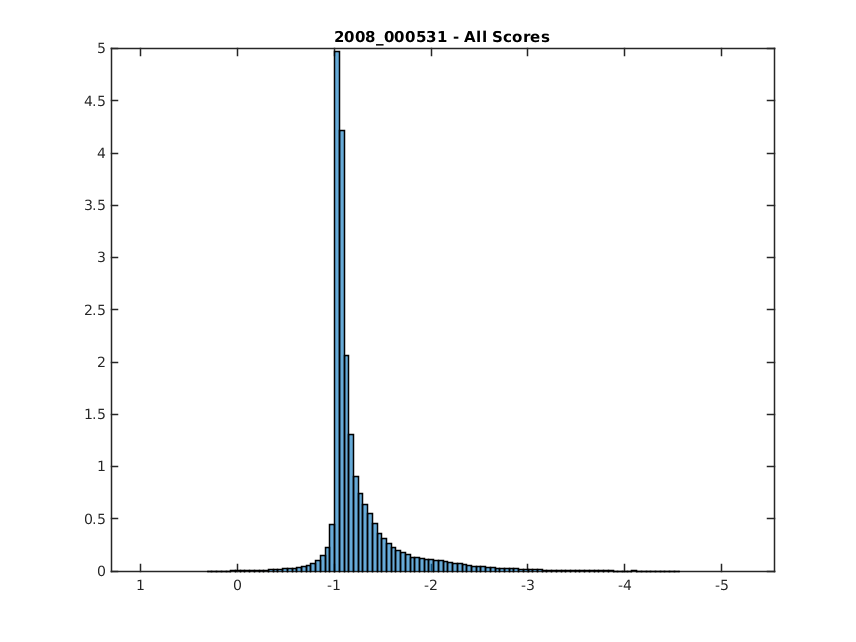
\includegraphics[width=\textwidth]{images/2008_000513_all.png}
\caption{Total score histogram of 2008\_000513}
\end{subfigure}%
\begin{subfigure}{0.5\textwidth}
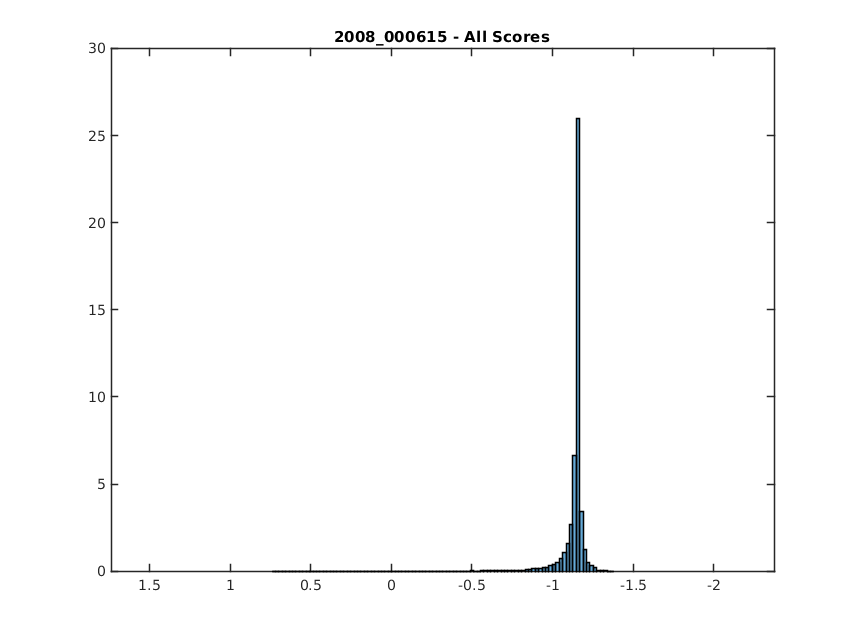
\includegraphics[width=\textwidth]{images/2008_000615_all.png}
\caption{Total score histogram of 2008\_000615}
\end{subfigure}

\begin{subfigure}{0.5\textwidth}
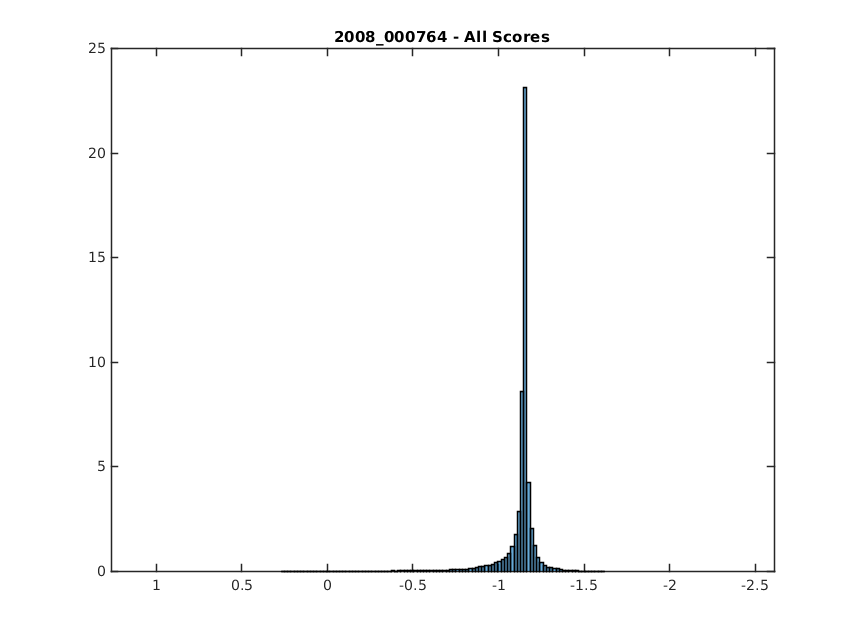
\includegraphics[width=\textwidth]{images/2008_000764_all.png}
\caption{Total score histogram of 2008\_000764}
\end{subfigure}%
\begin{subfigure}{0.5\textwidth}
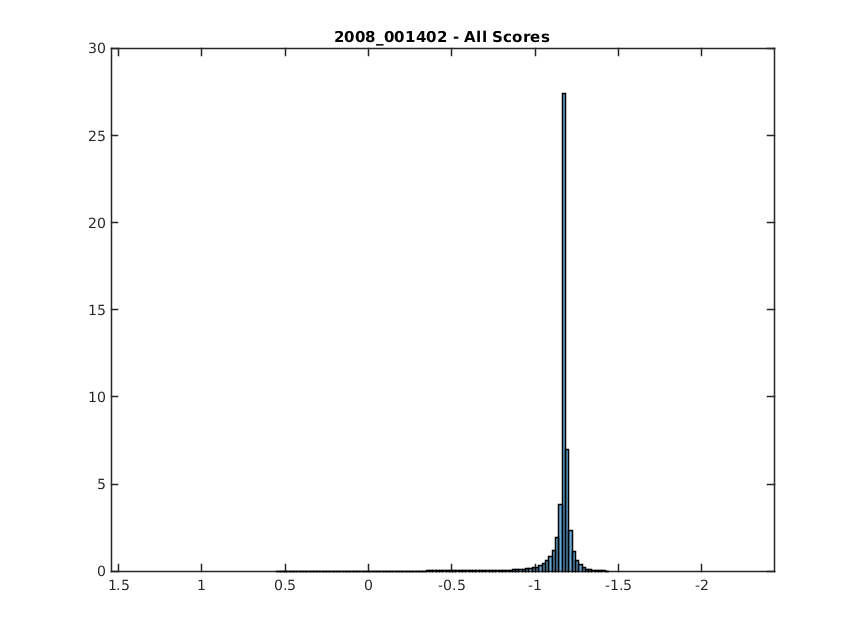
\includegraphics[width=\textwidth]{images/2008_001402_all.png}
\caption{Total score histogram of 2008\_001402}
\end{subfigure}
\caption[Score histograms]{Resulting unnormalized score histograms of different query images. The histogram shows all calculated scores of an image database consisting of 50 images based on a single query image respectively. Higher scores are on the left side, lower ones on the right side of each figure. The peak represents almost always false ``positive'' patches (as no normalization was done, the results are neither positive nor negative, some are just more likely true positive than others).}
\label{fig:score_histograms}
\end{figure}

As one will see in \figref{score_histograms}, this would fit for the most pictures used during the testing. The majority of windows is located at the same score, whereas windows with a score above the mean are closely located to the desired image part.
% gaussian fit + rho adjust
This additional normalization obviously increases the computation effort as it had to be done separately for each image in the database (after computing the scores for each window in the image). Therefore an approximation was applied by normalizing the scores in relation to the query image. To normalize the scores, a Gaussian curve is fitted onto the scored query image windows. By shifting the curve by $3\sigma$ into the direction of the highest scores, the relevant (positive) scores where pulled up near to one, whereas the negative scores get pushed down to zero. The resulting curve is then applied to all scores. This approximated normalization enabled us to produce comparable scores and therefore exclude whole images from the query results. An example could be seen in \figref{score_gauss_fit}.

\begin{figure}
\centering
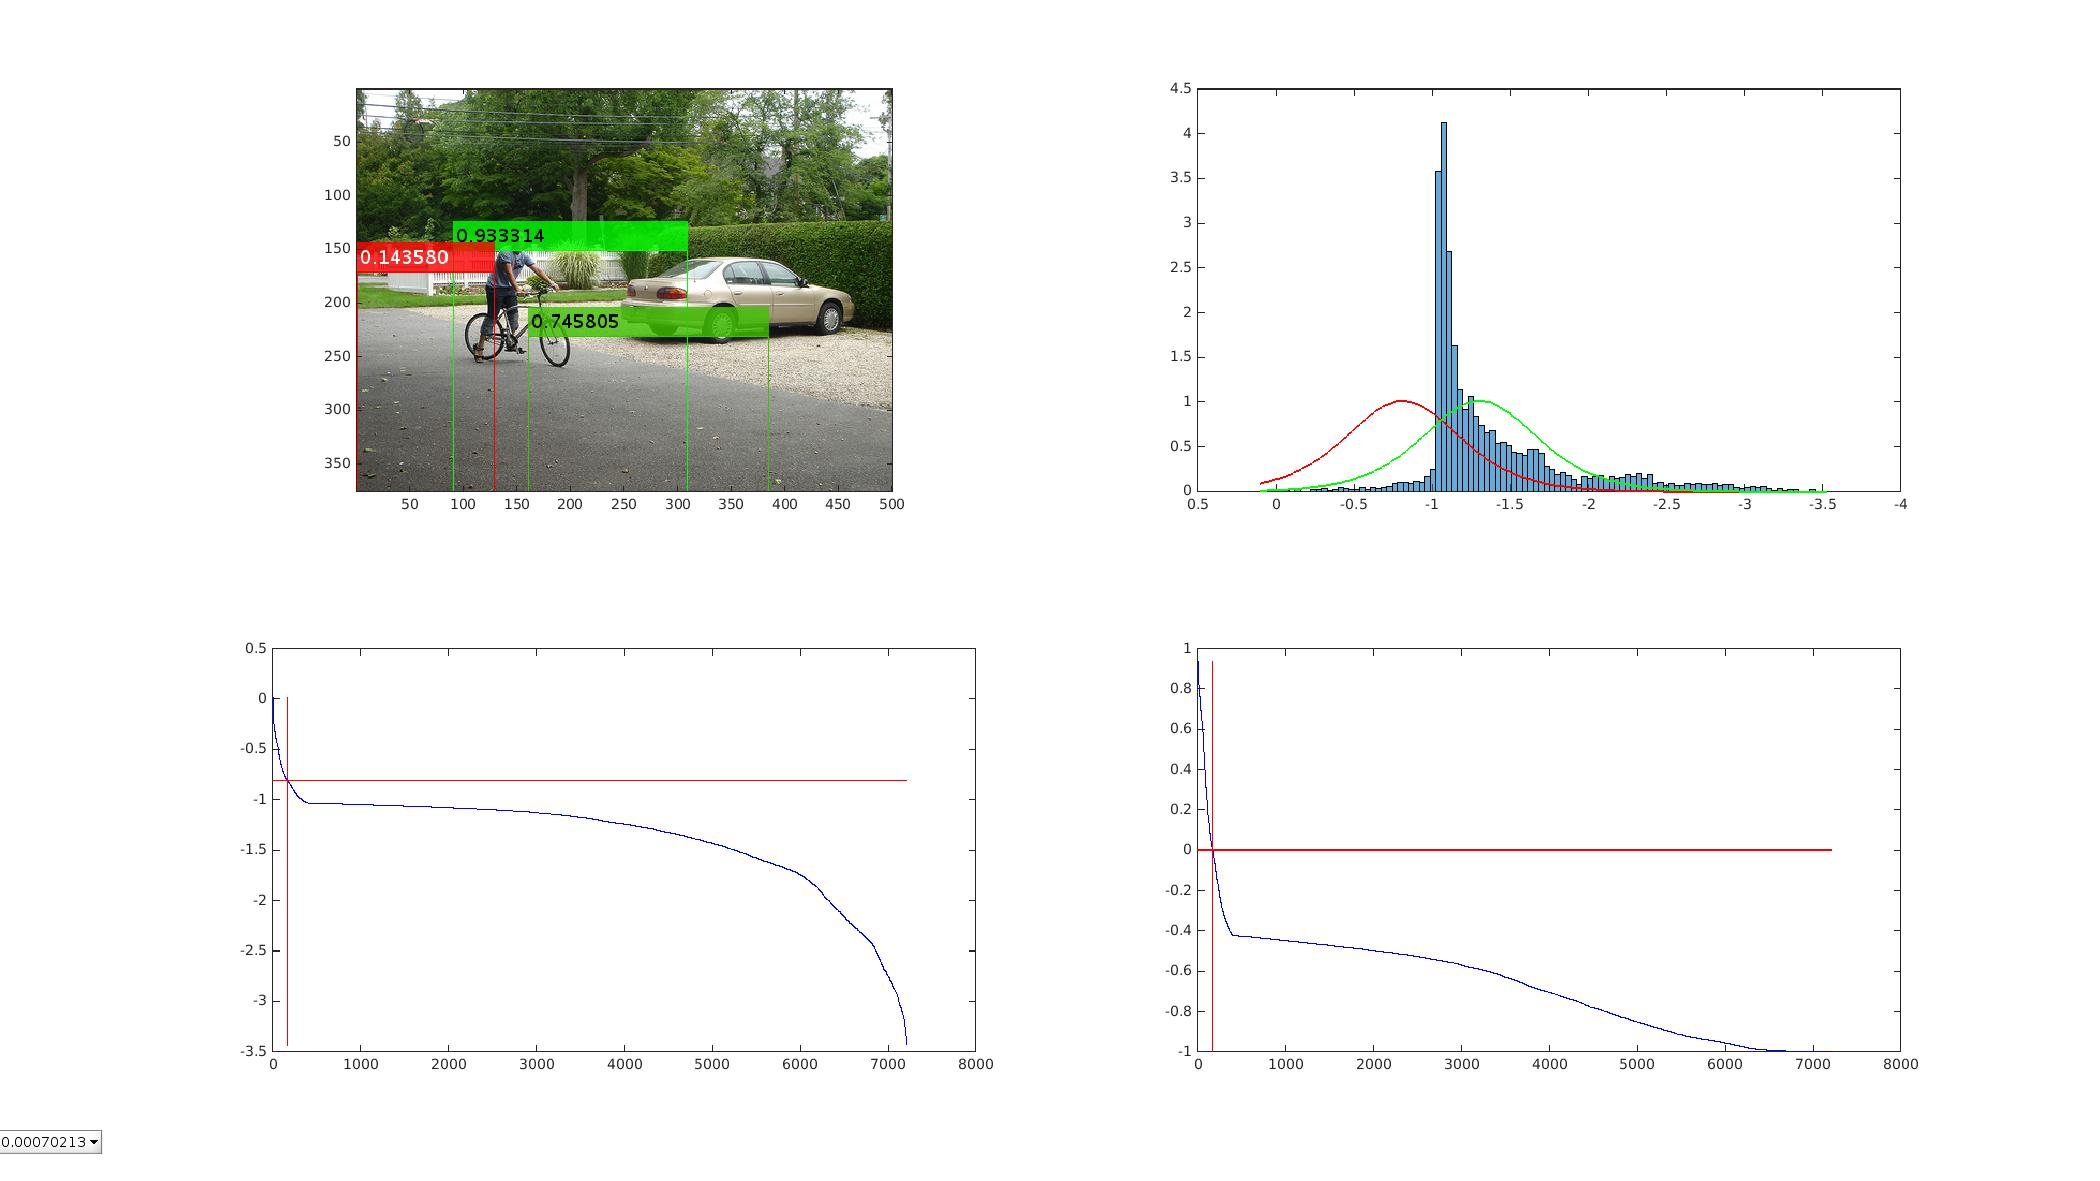
\includegraphics[width=\linewidth]{images/score_gauss_fit}
\caption{Gaussian fit to normalize \ac{SVM} scores}
\label{fig:score_gauss_fit}
\end{figure}


Another approach was to create a per image $svm_\rho$ value (comparable to the mean threshold) to orientate the scores at a common center point, but it turned out that the effort were to high compared to the performance gain.

After the score computation and normalization, a non maximum suppression was applied to minimize the output of similar, near located windows.
During the experiments, two non maximum suppression techniques were used and evaluated.

The first one is constructed by the union of the areas to compare (\ref{eqn:nonmax_union})

\begin{equation}
\frac{\text{area}(A \cap B)}{\text{area}(A \cup B)}
\label{eqn:nonmax_union}
\end{equation}

This technique computes the ratio between the common and total area of two bounding boxes $A$ and $B$. If this ratio has a value higher than $0.5$, the bounding box $B$ would be removed from the result list.

The second technique is based on \eqnref{nonmax_min}. This variant removes much more bounding boxes if they are enclosed by others, as only the area of smallest bounding box is used as the denominator. The previous technique removes only enclosed bounding boxes which are at least half as big as their enclosing boxes.

\begin{equation}
\frac{\text{area}(A \cap B)}{\min(\text{area}(A), \text{area}(B))}
\label{eqn:nonmax_min}
\end{equation}

The current algorithm produced the best results with the second technique, as it reduces the repetition of many positive windows showing only a single bicycle wheel. As they would not cover 50\% of the window enclosing the whole bicycle, they appear as new matches in the result list by using the first technique. Depending on the query image, it could be useful to switch between the suppression techniques as it could be desired to get smaller matches enclosed by a bigger one (for example children in front of their parents).

The downside of the second approach is that most of the time bigger windows are selected over the smaller ones. This produces good results if the image database contains a large representation of the query part, but not as accurate results otherwise.
